% Informe final (tipo paper, formato IEEE conference) — 1INF52 Deep Learning, PUCP 2026-2
% Compilar en Overleaf o local con: pdflatex x2 (las figuras se leen de ../figures/).
% En Overleaf: subir este .tex y la carpeta figures/ al mismo nivel, y cambiar \graphicspath a {figures/}.
% Todas las cifras provienen de results/C*.csv y results/E3_corridas/ (generados por scripts/E3_analisis.py).
\documentclass[conference,a4paper]{IEEEtran}
\usepackage[utf8]{inputenc}
\usepackage[T1]{fontenc}
\usepackage[spanish,es-noquoting,es-tabla]{babel}
\usepackage{amsmath,amssymb}
\usepackage{graphicx}
\usepackage{booktabs}
\usepackage{multirow}
\usepackage{xcolor}
\usepackage[hidelinks]{hyperref}
\graphicspath{{../figures/}}
\newcommand{\pend}[1]{\textcolor{red}{[PENDIENTE: #1]}}

\begin{document}

\title{¿Adaptar o congelar? LoRA sobre DINOv2 para clasificar cobertura del suelo en regiones geográficas no vistas}

\author{
\IEEEauthorblockN{Alfredo Jiménez, Jhonatan Davila, Italo Ramos}
\IEEEauthorblockA{Facultad de Ciencias e Ingeniería, Pontificia Universidad Católica del Perú (PUCP), Lima, Perú\\
1INF52 Deep Learning, 2026-2 \quad Grupo 4}
}

\maketitle

\begin{abstract}
Los modelos fundacionales de visión como DINOv2 se suelen transferir a imágenes satelitales con el backbone congelado (\emph{linear probing}). Adaptar la representación con LoRA mejora la clasificación en la distribución de entrenamiento, pero podría ajustarse a las regiones vistas y perder ventaja en regiones nuevas. Estudiamos esa hipótesis (H2) en EuroSAT RGB con DINOv2 ViT-S/14 y LoRA de rango 8 en las proyecciones Q y V de los dos últimos bloques (24{,}576 parámetros, 0{,}11\,\% del backbone). Construimos una partición geográfica por bloques espaciales a partir de las coordenadas de EuroSAT MS, que permite evaluar el mismo modelo en regiones vistas (\emph{test dentro}) y reservadas (\emph{test fuera}), y fijamos la regla de decisión antes de ejecutar. Con 3 semillas, ambos modelos caen al pasar a regiones nuevas (7{,}2 pts de macro-F1 el congelado, 5{,}9 pts LoRA), pero la ventaja de LoRA \emph{aumenta} de +0{,}9 pts dentro a +2{,}2 pts fuera, con el mismo signo en las 3 semillas y McNemar exacto $p<10^{-6}$ en cada una. H2 se rechaza: en este caso, adaptar los bloques profundos corrige un desajuste de dominio común a todas las regiones en lugar de sobreajustarse a las de entrenamiento. La mejora se concentra en vegetación herbácea, cultivos permanentes, carreteras y ríos.
\end{abstract}

\begin{IEEEkeywords}
DINOv2, LoRA, ajuste eficiente en parámetros, teledetección, EuroSAT, generalización geográfica, validación espacial.
\end{IEEEkeywords}

\section{Introducción}
DINOv2~\cite{oquab2024} es un Vision Transformer (ViT)~\cite{dosovitskiy2021} entrenado sin etiquetas sobre 142 millones de imágenes naturales; sus autores reportan que sus \emph{features} congeladas transfieren bien con un clasificador lineal. Las imágenes Sentinel-2 son distintas: vista cenital, unos 10\,m por píxel, texturas repetitivas y ningún objeto central. Entre las opciones para adaptar el modelo, LoRA~\cite{hu2022} entrena solo una actualización de rango bajo sobre pesos congelados y, una vez fusionada, no cambia el costo de inferencia.

Un clasificador de cobertura del suelo se entrena con unas regiones y se usa en otras, donde cambian cultivos, suelo y vegetación. Una partición aleatoria de EuroSAT~\cite{helber2019} sobreestima esa generalización, porque teselas vecinas, casi idénticas, caen en entrenamiento y prueba~\cite{roberts2017}. Nuestra pregunta es: \textbf{¿añadir LoRA a DINOv2 mejora la clasificación en regiones geográficas no vistas frente a DINOv2 congelado?} Planteamos dos hipótesis: H1, LoRA mejora el macro-F1 en la partición interna; y H2, en regiones reservadas ambos modelos caen y la ventaja de LoRA se reduce, porque parte de ella vendría de ajustarse a las regiones de entrenamiento.

Contribuciones: (i) un análisis del costo y de las representaciones de DINOv2 ViT-S/14 que motiva dónde intervenir; (ii) una partición geográfica por bloques espaciales de EuroSAT, construida a partir de las coordenadas de EuroSAT MS, con un \emph{test dentro} y un \emph{test fuera} para el mismo modelo; (iii) una comparación controlada con 3 semillas, McNemar exacto y una regla de decisión fijada antes de ejecutar; y (iv) ablaciones de rango, profundidad y proyecciones en ambas particiones, con predicciones registradas antes de correrlas. El código, las particiones, las 20 corridas y el cuaderno de decisiones están en el repositorio del proyecto.

\section{Trabajos relacionados}
\textbf{Transferencia de modelos fundacionales.} El protocolo de \emph{linear probing} de DINOv2 concatena el token de clase y la media de los tokens de parche~\cite{oquab2024}. Darcet \emph{et al.}~\cite{darcet2024} describen tokens de norma atípica en ViT sin registros. \textbf{Ajuste eficiente en parámetros.} LoRA~\cite{hu2022} obtiene sus mejores resultados, con presupuesto fijo, adaptando $W_q$ y $W_v$; Yosinski \emph{et al.}~\cite{yosinski2014} muestran que las capas profundas son las más específicas de la tarea original. \textbf{EuroSAT y validación espacial.} EuroSAT~\cite{helber2019} tiene 27{,}000 teselas de 34 países; una ResNet-50 ajustada por completo alcanza 98{,}57\,\% de \emph{accuracy} en RGB con partición aleatoria. Roberts \emph{et al.}~\cite{roberts2017} recomiendan bloques espaciales para datos con autocorrelación espacial, que es la estrategia que seguimos.

\section{Metodología}
\subsection{Datos y particiones}
Usamos EuroSAT RGB (10 clases, 64$\times$64\,px). Cada tesela se redimensiona a 224\,px (bicúbico, sin recorte central, que eliminaría el 23\,\% de la escena) y se normaliza con las estadísticas de ImageNet, como en el preentrenamiento.

\textbf{Partición interna:} estratificada 70/15/15 con semilla 42 (18{,}900/4{,}050/4{,}050), idéntica a la del E2.

\textbf{Partición geográfica:} las teselas RGB no tienen coordenadas, pero sus pares de EuroSAT MS (mismo nombre de archivo) son GeoTIFF georreferenciados. Verificamos el emparejamiento 1:1 de las 27{,}000 teselas y tomamos el centro de cada una en WGS84. Proyectamos a ETRS89-LAEA (EPSG:3035) y agrupamos con K-means. Regiones completas, distintas entre sí, forman la validación y el \emph{test fuera} (cada una entre 12 y 18\,\% del total); cada clase debe tener al menos el 5\,\% de sus imágenes en ambas. Entre las asignaciones válidas de 20{,}000 intentos se elige la más cercana a 15/15. De las regiones restantes se separa un \emph{test dentro} aleatorio estratificado (10\,\% del total); el resto es entrenamiento. El orden de respaldo si no hay solución ($K{=}12\rightarrow15\rightarrow20$, luego mínimo 3\,\%) se fijó antes de ejecutar; con $K{=}12$ no hubo asignación válida y se usó $K{=}15$. Resultado: 15{,}383 entrenamiento, 4{,}754 validación, 2{,}700 \emph{test dentro} y 4{,}163 \emph{test fuera}. El \emph{test fuera} son tres regiones: dos en Europa central (centros aprox.\ 18{,}5$^\circ$E 52{,}2$^\circ$N y 16{,}9$^\circ$E 48{,}0$^\circ$N) y una en el Mediterráneo oriental (33{,}0$^\circ$E 34{,}9$^\circ$N). La distancia mediana de una imagen de \emph{test fuera} a la imagen de entrenamiento más cercana es 492\,km (mínimo 12{,}4\,km), frente a 0{,}9\,km en \emph{test dentro}.

\subsection{Modelo y análisis del modelo base}
DINOv2 ViT-S/14 sin registros (\texttt{facebook/dinov2-small}) tiene 22{,}056{,}576 parámetros en 12 bloques iguales ($d{=}384$, 6 cabezas, MLP de 1{,}536). Medimos 12{,}25\,GFLOPs por imagen a 224\,px, igual a la fórmula analítica; la atención cuadrática es el 9{,}9\,\% (30{,}6\,\% a 448\,px). En una Tesla T4 la latencia es 8{,}9\,ms con batch 1 (fp32) y el throughput llega a 854\,img/s con batch 128 (fp16). Un PCA de los tokens muestra que el bloque 4 codifica sobre todo la posición del parche, mientras que en el bloque 12 los tokens se agrupan por clase de escena; el campo receptivo efectivo~\cite{luo2016} es global desde el bloque 1. Esto motiva intervenir en los bloques finales.

\subsection{Condiciones comparadas}
\textbf{Línea base (\emph{linear probing}):} backbone congelado; representación [CLS; media de parches] tras la norma final (768 dimensiones) y una capa lineal de 7{,}690 parámetros, entrenada sobre \emph{embeddings} precalculados.
\textbf{LoRA:} en Q y V de los bloques 11 y 12, $W'=W+\frac{\alpha}{r}BA$, con $r{=}\alpha{=}8$, $B{=}0$ al inicio (el modelo parte exactamente del congelado) y $A$ con inicialización Kaiming uniforme; 24{,}576 parámetros entrenables más la cabeza. Tras entrenar, $BA$ se fusiona en $W$ sin costo de inferencia.
\textbf{Presupuesto idéntico:} AdamW~\cite{loshchilov2019} (tasa $10^{-3}$, \emph{weight decay} $10^{-4}$), batch 64, 8 épocas, selección por el mejor macro-F1 de validación; precisión mixta fp16 en GPU. El conjunto de prueba no interviene en ninguna decisión.

\subsection{Protocolo de evaluación}
Métrica principal: macro-F1 (las clases tienen entre 2{,}000 y 3{,}000 imágenes). Cada comparación base vs.\ LoRA se repite con las semillas 42, 0 y 1 (las particiones no cambian con la semilla). La significancia frente al ruido del conjunto de prueba se mide con McNemar exacto~\cite{mcnemar1947} sobre predicciones pareadas. Para H2 definimos, por semilla y condición, la \emph{caída} = macro-F1(\emph{test dentro}) $-$ macro-F1(\emph{test fuera}) y la \emph{ventaja} de LoRA = macro-F1(LoRA) $-$ macro-F1(base). La regla, registrada el 24/11/2026 antes de ejecutar, usa la media de las 3 semillas: \emph{se cumple} la predicción de H2 si la caída está entre 3 y 10 pts en ambas condiciones y la ventaja fuera es $\le{+}0{,}5$ pts; \emph{se rechaza} si alguna caída es $<1$ pt o la ventaja fuera es $\ge{+}1{,}3$ pts; en otro caso es intermedio. Solo se afirma una dirección si las 3 semillas tienen el mismo signo.

\subsection{Ablaciones}
Con la semilla 42 y en ambas particiones: rango $r\in\{4,16\}$ ($\alpha{=}r$), LoRA en los 4 últimos bloques (9--12) y solo Q. Cada una tiene una predicción numérica y un criterio de rechazo registrados antes de ejecutar. Con una semilla, diferencias menores a $\sim$0{,}6 pts (partición interna) no se distinguen del ruido.

\section{Resultados}
\subsection{Partición interna (H1)}
La Tabla~\ref{tab:semillas} resume las 3 semillas. LoRA mejora el macro-F1 en las tres (+1{,}19, +1{,}32 y +2{,}06 pts; media +1{,}52 $\pm$ 0{,}47) con McNemar $p\le2\times10^{-4}$ en cada semilla. H1 se confirma.

\begin{table}[t]
\centering
\caption{Macro-F1 (\%) por conjunto de prueba, media $\pm$ desviación de 3 semillas. $\Delta$ = LoRA $-$ base.}
\label{tab:semillas}
\begin{tabular}{@{}lccc@{}}
\toprule
Conjunto & Base & LoRA & $\Delta$ \\
\midrule
Interna (test aleatorio) & 95{,}66 $\pm$ 0{,}19 & 97{,}18 $\pm$ 0{,}39 & +1{,}52 $\pm$ 0{,}47 \\
Geográfica, test dentro & 96{,}40 $\pm$ 0{,}22 & 97{,}32 $\pm$ 0{,}19 & +0{,}92 $\pm$ 0{,}36 \\
Geográfica, test fuera & 89{,}25 $\pm$ 0{,}88 & 91{,}45 $\pm$ 0{,}57 & +2{,}20 $\pm$ 1{,}00 \\
\bottomrule
\end{tabular}
\end{table}

\subsection{Regiones no vistas (H2)}
Ambos modelos pierden rendimiento en regiones reservadas (Fig.~\ref{fig:geo}): la caída media es 7{,}15 $\pm$ 0{,}68 pts para la base y 5{,}87 $\pm$ 0{,}40 pts para LoRA. El cambio de distribución es real y similar en magnitud a lo previsto (3--10 pts). Sin embargo, la ventaja de LoRA no se reduce: pasa de +0{,}92 pts en \emph{test dentro} a +2{,}20 pts en \emph{test fuera} (+1{,}70, +3{,}35 y +1{,}56 por semilla), siempre positiva, con McNemar exacto $p<10^{-6}$ en cada semilla (Tabla~\ref{tab:mcnemar}). Como la ventaja fuera supera el umbral de +1{,}3 pts, \textbf{la predicción de H2 se rechaza}. Comparando de forma secundaria con los modelos de la partición interna, la diferencia entre su test aleatorio y el \emph{test fuera} de los modelos geográficos es de 6{,}41 pts (base) y 5{,}73 pts (LoRA): la partición aleatoria sobreestima en unos 6 pts el rendimiento en regiones nuevas.

\begin{figure}[t]
\centering
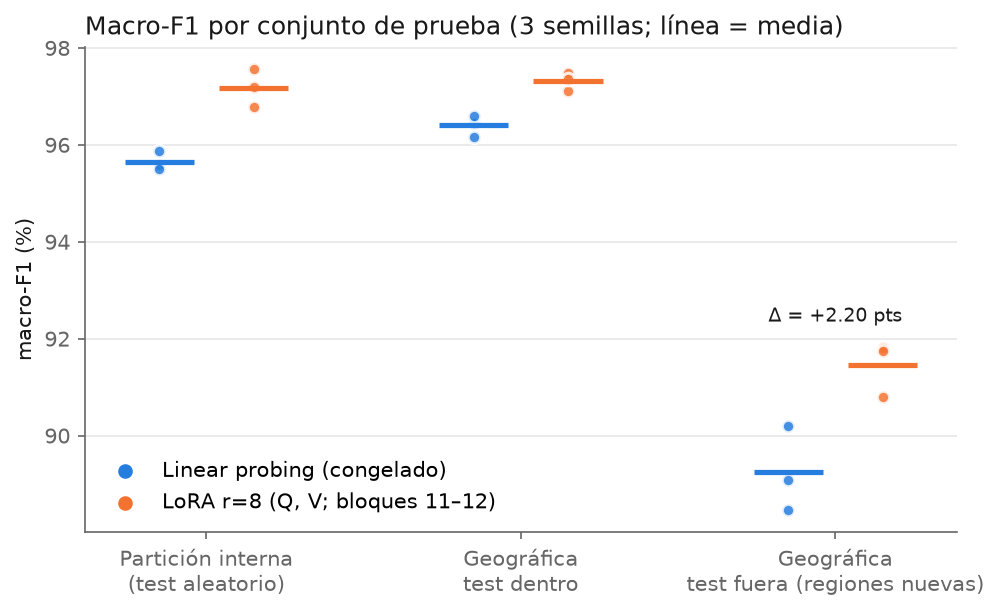
\includegraphics[width=\columnwidth]{C4_interno_vs_geo.png}
\caption{Macro-F1 por conjunto de prueba. Puntos: semillas; línea: media. La ventaja de LoRA crece en regiones no vistas.}
\label{fig:geo}
\end{figure}

\begin{table}[t]
\centering
\caption{McNemar exacto base vs.\ LoRA en \emph{test fuera}: imágenes que solo acierta cada modelo.}
\label{tab:mcnemar}
\begin{tabular}{@{}cccc@{}}
\toprule
Semilla & Solo base & Solo LoRA & $p$ \\
\midrule
42 & 67 & 161 & $4{,}2\times10^{-10}$ \\
0 & 95 & 211 & $2{,}9\times10^{-11}$ \\
1 & 77 & 153 & $6{,}1\times10^{-7}$ \\
\bottomrule
\end{tabular}
\end{table}

\textbf{¿Dónde gana LoRA fuera de las regiones de entrenamiento?} La Fig.~\ref{fig:clases} muestra el F1 por clase. Las mayores ventajas fuera están en vegetación herbácea (+5{,}2 pts), cultivos permanentes (+4{,}4), carreteras (+4{,}1) y ríos (+4{,}0). Carreteras y ríos ya eran las clases con más ganancia en la partición interna. La caída por región se concentra en las clases agrícolas: cultivos permanentes pierde 34 pts (base) y 31 pts (LoRA), y pastizales unos 12 pts en ambos, mientras que bosque, agua e industria casi no cambian. Es decir, el cambio de región afecta sobre todo a clases cuyo aspecto depende de prácticas agrícolas locales, y LoRA no lo elimina, pero lo reduce en vegetación herbácea (caída de 11{,}9 a 6{,}8 pts) y en cultivos anuales (8{,}1 a 5{,}8). Por región de \emph{test fuera}, LoRA mejora en las tres (+1{,}1 a +1{,}8 pts de macro-F1); la región mediterránea es la más difícil para ambos (47{,}5 vs.\ 49{,}3), aunque solo contiene 5 clases y 424 imágenes.

\begin{figure*}[t]
\centering
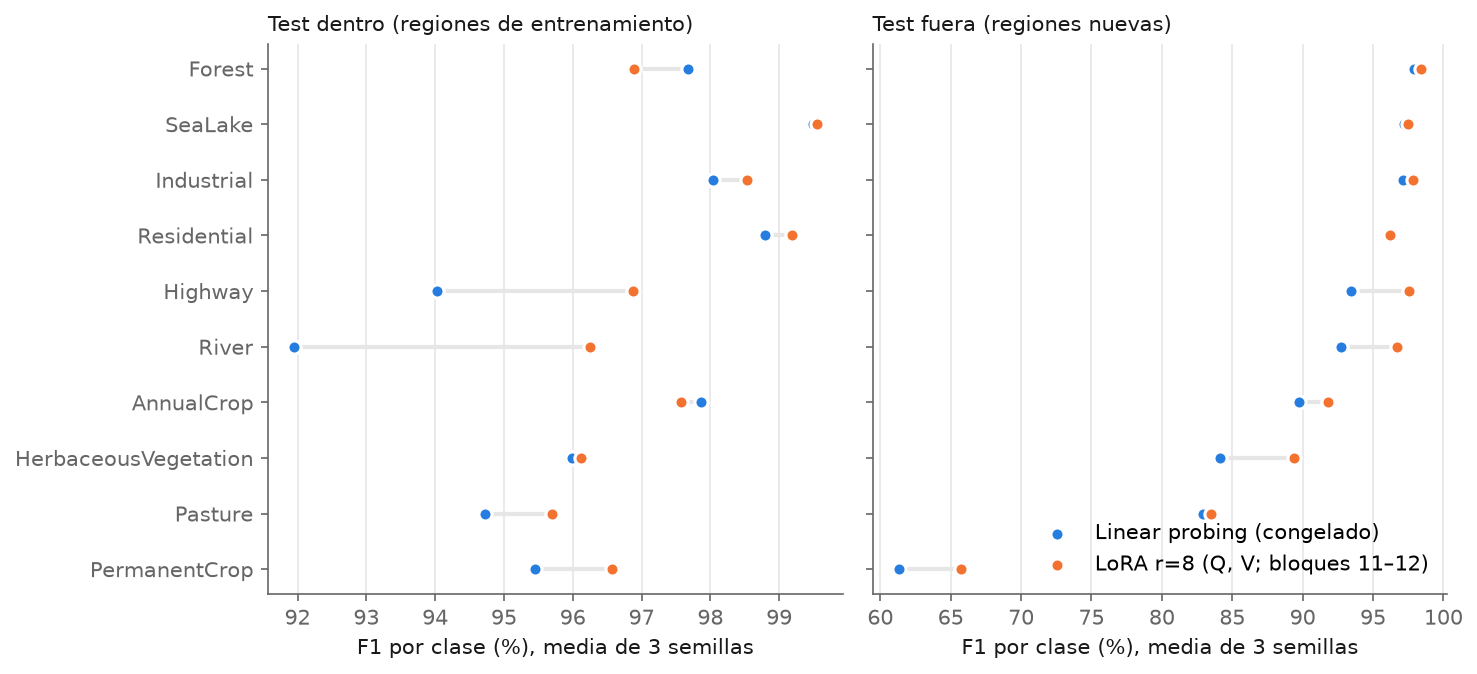
\includegraphics[width=0.85\textwidth]{C5_f1_por_clase_geo.png}
\caption{F1 por clase (media de 3 semillas) en \emph{test dentro} y \emph{test fuera}. Las clases agrícolas concentran la caída; LoRA gana sobre todo en vegetación herbácea, cultivos permanentes, carreteras y ríos.}
\label{fig:clases}
\end{figure*}

\subsection{Ablaciones}
La Tabla~\ref{tab:ablaciones} compara cada variante con LoRA $r{=}8$, Q+V, bloques 11--12 (semilla 42). En la partición interna, adaptar los 4 últimos bloques es la única variante con una diferencia mayor que el ruido (+1{,}19 pts); la predicción (+0{,}1 a +0{,}5) se rechaza por subestimar la mejora. Solo Q rindió +0{,}45 pts sobre Q+V, contra la predicción de una caída de 0{,}2--0{,}6 pts (se rechaza, aunque la diferencia está dentro del ruido de una semilla). El rango casi no importa ($r{=}16$: +0{,}08; $r{=}4$: +0{,}49), coherente con~\cite{hu2022}. En la partición geográfica, 4 bloques es también la mejor variante fuera de las regiones de entrenamiento (+1{,}48 pts) y \emph{reduce} la caída en 0{,}69 pts; habíamos predicho lo contrario (más caída, por alterar \emph{features} más genéricas), así que esa predicción se rechaza. Rango y solo Q apenas cambian la caída ($\le$0{,}5 pts).

\begin{table}[t]
\centering
\caption{Ablaciones (semilla 42), macro-F1 (\%). $\Delta$: diferencia con LoRA $r{=}8$ Q+V bloques 11--12. Interna: test aleatorio; geográfica: test fuera y $\Delta$ de la caída (dentro $-$ fuera).}
\label{tab:ablaciones}
\setlength{\tabcolsep}{4pt}
\begin{tabular}{@{}lcccc@{}}
\toprule
& \multicolumn{2}{c}{Interna} & \multicolumn{2}{c}{Geográfica} \\
\cmidrule(lr){2-3}\cmidrule(lr){4-5}
Variante & F1 & $\Delta$ & F1 fuera ($\Delta$) & $\Delta$ caída \\
\midrule
Referencia ($r{=}8$, Q+V, b.\ 11--12) & 96{,}78 & -- & 90{,}79 & -- \\
$r=4$ & 97{,}27 & +0{,}49 & 90{,}54 ($-$0{,}25) & $-$0{,}09 \\
$r=16$ & 96{,}86 & +0{,}08 & 90{,}97 (+0{,}18) & +0{,}46 \\
Bloques 9--12 & 97{,}97 & +1{,}19 & 92{,}27 (+1{,}48) & $-$0{,}69 \\
Solo Q & 97{,}24 & +0{,}45 & 90{,}60 ($-$0{,}19) & +0{,}30 \\
\bottomrule
\end{tabular}
\end{table}

\subsection{Costo}
Entrenar LoRA toma unos 500--580\,s por corrida en la T4, frente a unos 5\,s de la línea base una vez extraídos los \emph{embeddings} ($\sim$70\,s la primera vez). Tras fusionar $BA$ en $W$, el modelo tiene el mismo tamaño y la misma latencia que el original (4{,}43 vs.\ 4{,}41\,ms/imagen con batch 32).

\section{Discusión}
Esperábamos que la ventaja de LoRA fuera, en parte, sobreajuste a las regiones de entrenamiento, ya que su pérdida de entrenamiento llega a valores muy bajos. Los datos dicen lo contrario: la ventaja es mayor fuera que dentro y la caída de LoRA es menor que la de la base. Una lectura coherente con el análisis del modelo base es que el desajuste principal de DINOv2 con EuroSAT no es regional sino de dominio: vista cenital, baja resolución reescalada y texturas en lugar de objetos. Ese desajuste es común a todas las regiones y adaptar la atención de los bloques profundos lo corrige en todas. Que adaptar 4 bloques generalice aún mejor apunta en la misma dirección. Lo que sí es regional, la apariencia de los cultivos, sigue limitando a ambos modelos. El F1 de cultivos permanentes cae más de 30 pts sobre todo por falsos positivos: en regiones nuevas, vegetación herbácea y cultivos anuales se predicen como cultivos permanentes (89 y 68 imágenes por semilla con la base; 56 y 49 con LoRA). LoRA reduce los errores en \emph{test fuera} de 352 a 257 por semilla ($-$27\,\%), en gran parte en esas confusiones, pero no las elimina; el bosque oscuro confundido con agua ($\sim$11 por semilla) persiste en ambos (Fig.~\ref{fig:ejemplos}).

\begin{figure*}[t]
\centering
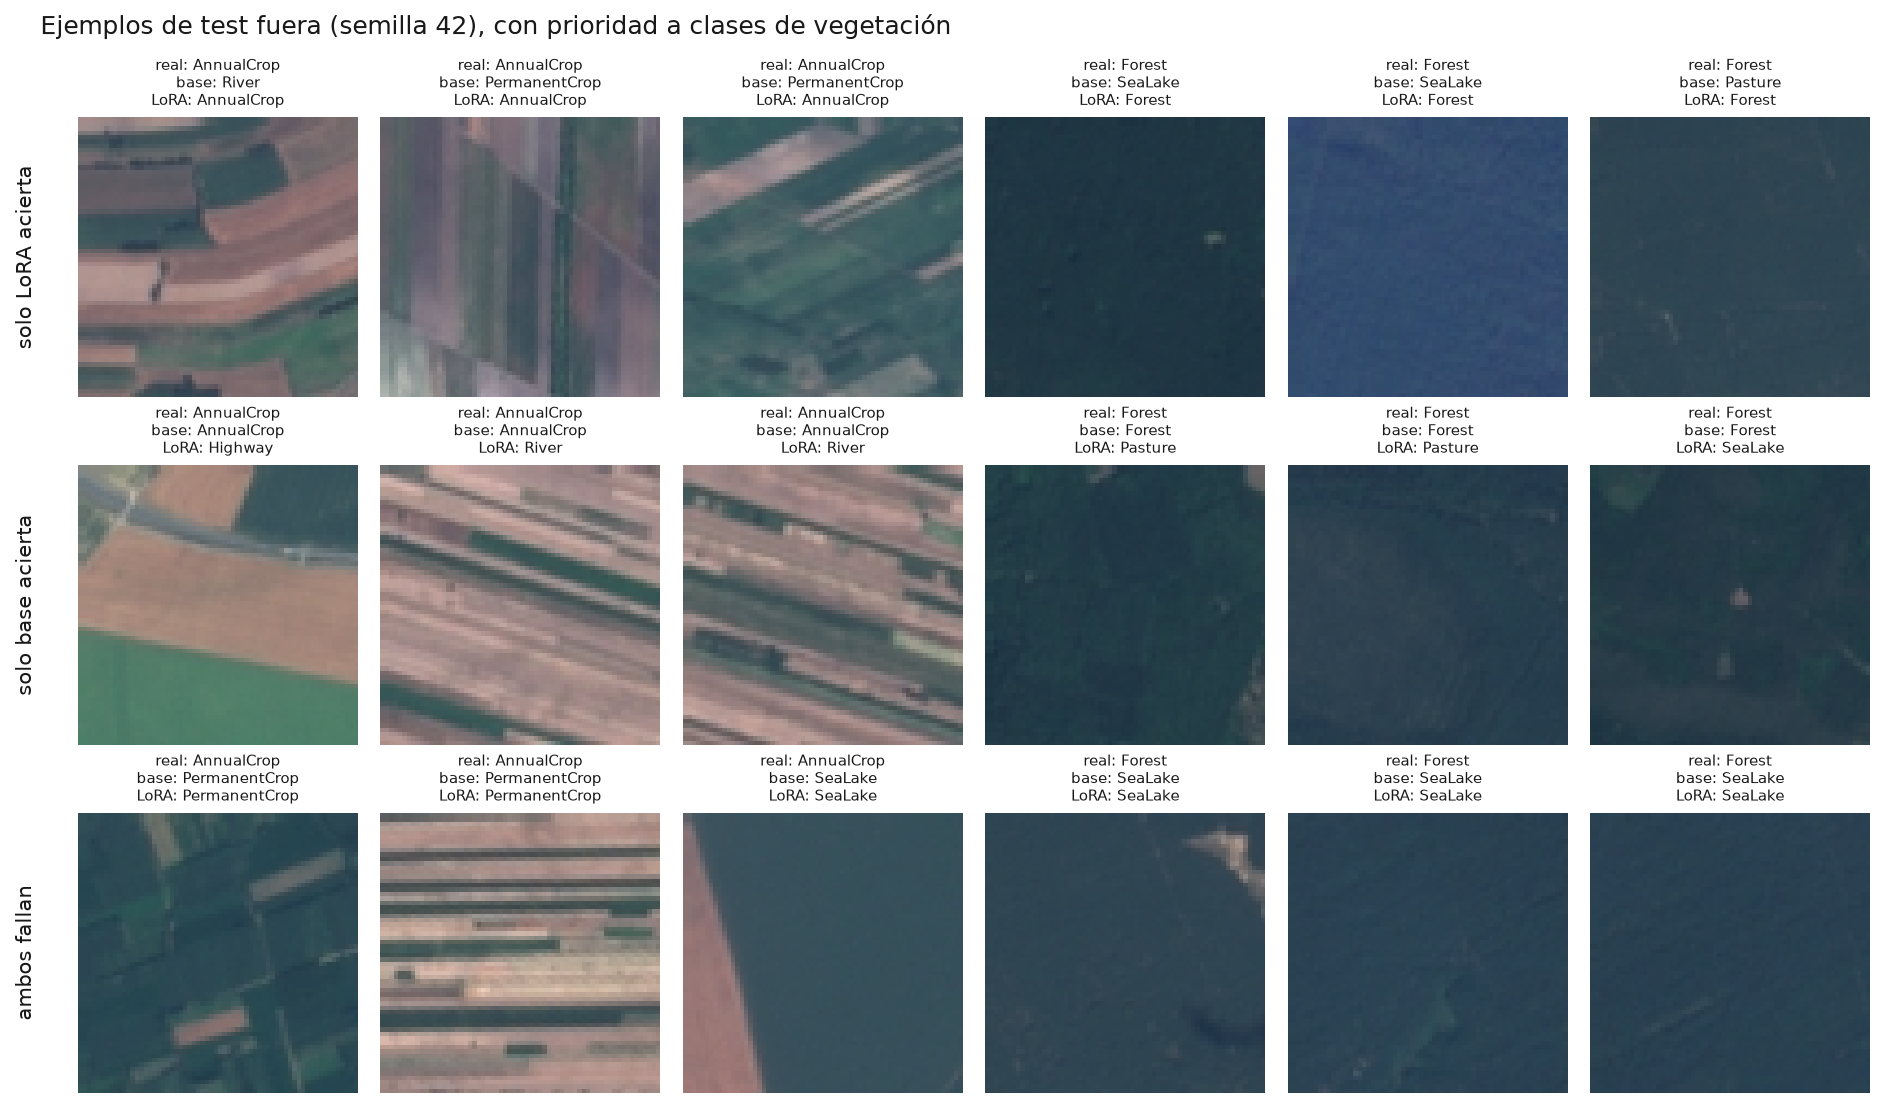
\includegraphics[width=0.85\textwidth]{C8_ejemplos_fallo_geo.png}
\caption{Ejemplos de \emph{test fuera} (semilla 42) donde solo LoRA acierta, solo la base acierta o ambos fallan.}
\label{fig:ejemplos}
\end{figure*}

\textbf{Amenazas a la validez.} (i) El \emph{test fuera} tiene solo tres regiones, dos de ellas en Europa central; otra partición podría dar otra magnitud de caída. (ii) Las ablaciones usan una semilla. (iii) No hubo búsqueda de hiperparámetros; ambos modelos usan el mismo presupuesto. (iv) Después de las corridas, una revisión de código encontró dos desviaciones del presupuesto del E2 en el entrenamiento de LoRA: se usó fp16 sin escalado de gradientes (\emph{GradScaler}) y la inicialización de $A$ no dependía de la semilla de la corrida. Las 6 corridas de la línea base no se ven afectadas. La validación de LoRA (semilla 42, partición interna: 97{,}46) reproduce la del E2 (97{,}52), lo que indica que el entrenamiento no quedó frenado; el test interno (96{,}78 vs.\ 97{,}14 en el E2) difiere en 0{,}36 pts, del orden del ruido. Una corrida de control con el código corregido \pend{resultado de la corrida de control: results/C11\_control\_correccion.csv}. (v) La partición geográfica se generó en la misma sesión, justo antes de entrenar, y no se commiteó antes; es determinista y se regeneró idéntica, imagen por imagen.

\section{Conclusiones}
En EuroSAT, adaptar DINOv2 ViT-S/14 con LoRA en Q y V de los dos últimos bloques (0{,}11\,\% de parámetros adicionales y sin costo de inferencia tras fusionar) mejora el macro-F1 en la partición interna (+1{,}5 pts) y aún más en regiones geográficas no vistas (+2{,}2 pts, consistente en 3 semillas). Ambos modelos pierden 6--7 pts al pasar a regiones nuevas, sobre todo en clases agrícolas, y la partición aleatoria sobreestima en unos 6 pts el rendimiento real en regiones nuevas. La hipótesis de que LoRA perdería su ventaja fuera de las regiones de entrenamiento se rechaza. Como trabajo futuro: más regiones de prueba (validación cruzada espacial con varios pliegues), más semillas en las ablaciones, adaptar más bloques y comparar con la variante con registros.

\section*{Reproducibilidad y uso de IA}
Las particiones (\texttt{splits/}), las 20 corridas con sus predicciones (\texttt{results/E3\_corridas/}), el código (\texttt{src/eurosat\_lora/}) y el cuaderno de decisiones con las predicciones previas están en el repositorio. Se usaron asistentes de IA (Claude, Antigravity) para el diseño del protocolo, el código, la revisión de código y la redacción; el detalle y lo que revisó el equipo está en \texttt{DESIGN\_LOG.md}, sección~4.

\begin{thebibliography}{99}
\bibitem{oquab2024} M. Oquab, T. Darcet, T. Moutakanni \emph{et al.}, ``DINOv2: Learning robust visual features without supervision,'' \emph{Trans. Mach. Learn. Res.}, 2024.
\bibitem{dosovitskiy2021} A. Dosovitskiy \emph{et al.}, ``An image is worth 16x16 words: Transformers for image recognition at scale,'' in \emph{Proc. ICLR}, 2021.
\bibitem{hu2022} E. J. Hu \emph{et al.}, ``LoRA: Low-rank adaptation of large language models,'' in \emph{Proc. ICLR}, 2022.
\bibitem{helber2019} P. Helber, B. Bischke, A. Dengel, and D. Borth, ``EuroSAT: A novel dataset and deep learning benchmark for land use and land cover classification,'' \emph{IEEE J. Sel. Topics Appl. Earth Observ. Remote Sens.}, vol.~12, no.~7, pp.~2217--2226, 2019.
\bibitem{roberts2017} D. R. Roberts \emph{et al.}, ``Cross-validation strategies for data with temporal, spatial, hierarchical, or phylogenetic structure,'' \emph{Ecography}, vol.~40, no.~8, pp.~913--929, 2017.
\bibitem{darcet2024} T. Darcet, M. Oquab, J. Mairal, and P. Bojanowski, ``Vision transformers need registers,'' in \emph{Proc. ICLR}, 2024.
\bibitem{yosinski2014} J. Yosinski, J. Clune, Y. Bengio, and H. Lipson, ``How transferable are features in deep neural networks?'' in \emph{Proc. NeurIPS}, 2014.
\bibitem{luo2016} W. Luo, Y. Li, R. Urtasun, and R. Zemel, ``Understanding the effective receptive field in deep convolutional neural networks,'' in \emph{Proc. NeurIPS}, 2016.
\bibitem{loshchilov2019} I. Loshchilov and F. Hutter, ``Decoupled weight decay regularization,'' in \emph{Proc. ICLR}, 2019.
\bibitem{mcnemar1947} Q. McNemar, ``Note on the sampling error of the difference between correlated proportions or percentages,'' \emph{Psychometrika}, vol.~12, no.~2, pp.~153--157, 1947.
\end{thebibliography}

\end{document}
